\chapter{Stapelung von Signalen}
Das Stapeln von Signalereihen wird genutzt um ein besseres Signal zu Rausch Verhältnis (eng. \textsl{Signal-to-Noise Ratio}) des gewünschten Signals zu bekommen als auch bei der räumlichen Analyse von Signalen.
Die Stapelung der Signalreihen wird benutzt bei:
\begin{itemize}
\item Wiederholter Anregung des Input Signals\\
Z.B. in der Hammerschlagseismik oder Ultraschall.
\item Bündelung von Geophonen ($\rightarrow$ \textit{Geophone Group Interval})
\item Gruppierung von Quellen\\
Z.B. bei der Vibroseismik.
\item Stapelung von Seismogrammen\\
Wie bei der CMP Stapelung, reflektierte Wellen werden nach der \textit{Normal-Move-Out} (NMO) Korrektur gestapelt.
\end{itemize}

\section{Beispiele der Stapelung}
\subsubsection*{Beispiel}
Überlagerung zweier Signale mit gleicher Frequenz $\omega_0$, aber unterschiedlicher Phase.  Das ist ein einfaches Beispiel für eine Stapelung mit $t_i\not= 0$ und $n_i=0$. Die zwei Signale sind:
\begin{align*}
s_1(t) & =\cos(\omega_0 t+\varphi_1)\\
s_2(t) & =\cos(\omega_0 t+\varphi_2).
\end{align*}
Mit dem Additionstheorem ergibt die Überlagerung:
\begin{equation}
s_1(t)+s_2(t)=2 \cos \left(\omega_0 t + \frac {\varphi_1 + \varphi_2}{2}\right)\, \cos\left(\frac {\varphi_1 - \varphi_2}{2}\right).
\end{equation}
Das bedeutet die Frequenz ändert sich nicht. Die Phasenverschiebung wird gemittelt und es ergibt sich ein zeitunabhängiger Wichtungsfaktor, der von der Phasendifferenz abhängt. Für $\varphi_1-\varphi_2= \pi $ löschen sich die Signale gegenseitig aus.\\\\
Für eine Phasenverschiebung von $|\varphi_1-\varphi_2|\le \frac{\pi}{2}$ ($\Delta\varphi = \frac{\lambda}{4}$) gilt für den Wichtungsfaktor $\cos \left(\frac{\varphi_1-\varphi_2}{2} \right)\ge 0.7071$ und es liegt konstruktive Interferenz vor.\\ 

\subsubsection*{Beispiel}
Überlagerung zweier Signale mit unterschiedlicher Frequenz:
\begin{align*}
s_1(t) & = \cos(\omega_1 t)\\
s_2(t) &= \cos(\omega_2 t)
\end{align*}
Mit dem Additionstheorem folgt:
\begin{equation}
s_1(t)+s_2(t)= 2 \cos \left(\frac{\omega_1+\omega_2}{2}t\right)\, \cos \left(\frac{\omega_1-\omega_2}{2}t\right).
\end{equation}

Es ergibt sich eine Schwebung mit einer hochfrequenten Trägerfrequenz $\frac{\omega_1+\omega_2}{2}$ und einer niederfrequenten Amplitudenmodulation mit der Frequenz $f_A = \frac{1}{2\pi}\frac{\omega_1-\omega_2}{2}$. Interessant ist, dass zu den Zeitpunkten $\frac{n}{2f_A}+\frac{1}{4f_A}$ mit $n \in \mathbb{G}$ ein Phasensprung auftritt. Die Maxima der Einhüllenden sind ebenfalls $\frac{1}{2f_A}$ entfernt. Beachte: wird eine Fourieranalyse von diesem Signal gemacht, treten nur die Frequenzen $\omega_1$ und $\omega_2$ auf. Die Formulierung mit amplitudenmodulierter Trägerfrequenz ist jediglich äquivalent.\\ 

\subsubsection*{Beispiel}
Ein Signal soll zwei Frequenzen $\omega_1$ und $\omega_2$ enthalten: $s(t) = \cos (\omega_1t) + \cos(\omega_2t)$. Betrachtet wird die Überlagerung zweier zeitverschobener Signale:
\begin{align*}
s_1(t) &=s(t+t_1)\\
s_2(t) &=s(t+t_2)
\end{align*}

Mit dem Additionstheorem folgt:
\begin{multline}
s_1(t)+s_2(t)= 2 \cos \left(\omega_1 t +\omega_1\frac{t_1+t_2}{2}\right)\, \cos \left(\omega_1\frac{t_1-t_2}{2}\right)\\
+2 \cos \left(\omega_2 t +\omega_2\frac{t_1+t_2}{2}\right)\, \cos\left(\omega_2\frac{t_1-t_2}{2}\right).
\end{multline}

\begin{itemize}
\item Die Frequenzen $\omega_1$ und $\omega_2$ bleiben erhalten.
\item $\cos (\omega_1\frac{t_1-t_2}{2})=f_1$ und $ \cos(\omega_2\frac{t_1-t_2}{2})=f_2$ sind zeitunabhängige Wichtungsfaktoren für die beiden Frequenzen.
\item Für $\omega_1<\omega_2$ ist $f_1>f_2$, d.h. die Stapelung ist ein Tiefpass. Die Bedingung für konstruktive Interferenz ist für tiefe Frequenzen eher erfüllt als für hohe Frequenzen. 
\end{itemize}

\section{Beamforming}
Bei Beamforming sucht man die richtige Wellenzahlvektor $\vec{k}$ der einfallenden Erdbebenwelle in ein Array von Seismometern. Dabei wird die Stappelung von vielen Seismogrammen benutzt um den Wellenzahlvektor der einfallenden seismischen Welle zu bestimmen.\\
Ein Seismogramm $u(x,y,t)$ kann als Funktion der Zeit und des Ortes plus Rauschen dargestellt werden:
\begin{equation}
u(x,y,t) = s(t-t_{j})+m(x_{j},y_{j},t)
\end{equation}
Dabei ist $s(t-t_{j})$ das zeitverschobene Signal um $t_j$ und $m(x_{j},y_{j},t)$ das ortsabhängige gleichverteilte Rauschen.\\
Nun werden viele Slowness Vektoren berechnet. Für die wahre Slowness $\vec{p}$ gilt: 
\[
\vec{p} \approx \hat{\vec{p}}
\]
So ist die Zeitverschiebung ist der Station $j$ für einen Slowness Vektor $\hat{\vec{p}}$ relativ zum Zentrum des Arrays $\vec{r}$:
\begin{equation}
\hat{t}_{j}=\hat{\vec{p}} \vec{r}
\end{equation}
Durch Summieren für eine bestimmte Slowness $\hat{\vec{p}}$ über alle Stationen wird ein Beam $b(t)$ erzeugt:
\begin{equation}
 b(t) = \sum_{j=1}^{n} u( x_j,y_j,t+t_j)
\end{equation}
Wobei $j$ der Stationindex ist.\\
Alle Seismogramme werden mit einer bestimmten Slowness verschoben. Der Prozess wird für alle Langsamkeiten , $\hat{\vec{p}}$, durchgeführt. So kann die passende Wellenzahl der ankommenden Wellenfront wird ermittelt werden.
\begin{equation}
b(t) = M_s(t)+ \sum_{j=1}^n u( x_j,y_j,t+t_j)
\end{equation}
Dabei ist $M_s(t)$ die konstruktive Interferenz und
\[
\sum_{j=1}^n u( x_j,y_j,t+t_j)
\]
die destruktive Interferenz.
\begin{figure}[h!]
\centering
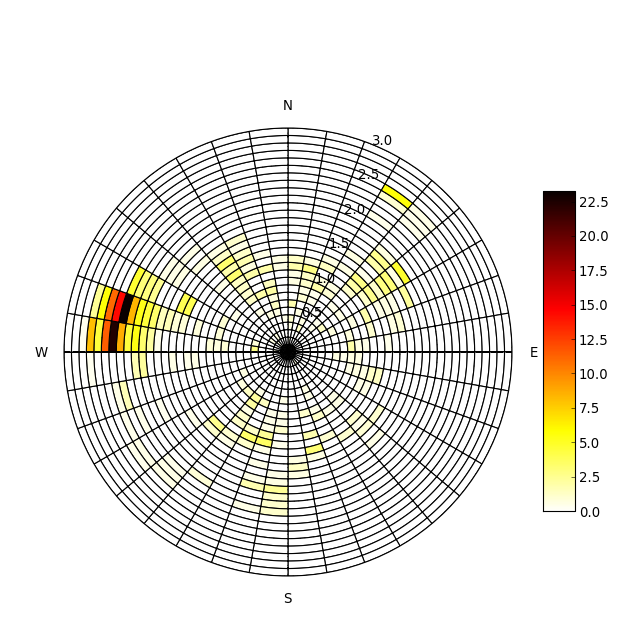
\includegraphics[width=.7\tw]{fig/05-Stapelung/beamforming_fk_analysis.png}
\caption{Beamforming Analyse von seismischen Wellen abgestrahlt von einer Hochhaussprengung in München. Aus ObsPy Gallerie (\url{http://docs.obspy.org/})}
\end{figure}

\subsection{Velocity Spectrum Analysis}
Die Richtung der ankommenden Wellenfront sei bekannt, aber der Betrag der Slowness  $|\vec{p}|$ und die Phasengeschwindigkeit $c_x$ seien unbekannt.
In diesem Fall kann die Geschwindigkeit-Spektrum-Analyse (eng. \textsl{Velocity Spectrum Analysis}) durchgeführt werden.\\
Dabei wird der Betrag der Slowness $|\hat{\vec{p}}|$, systematisch variiert, und jeweils wird ein Beam berechnet.
\[
Stack = f(\vert\hat{\vec{p}}\vert,t)
\]
Alle Hypothesen, jede Slowness, wird berechnet und erstellt daraus das Vespagramm.

\subsection{f-k-Analyse}
Die Frequenz-Wellenzahl Analyse kann auch berechnet werden um den Wellenzahlvektor zu berechnen.
Im Fall, das Geschwindigkeit und Richtung der Wellenfront unbekannt ist, kann eine Frequenz-Wellenzahl-Analyse durchgeführt werden. Dabei wird eine 3D-Fourier-Transformation durchgeführt:
\begin{equation}
u(k_{x},k_{y},\omega) = \iiint_{-\infty}^{\infty} u(x,y,t)\cdot e^{(-i(k_{x}x+k_{y}y+\omega t))} dxdyd\omega
\end{equation}
Das Modell (\textbf{für was?}) sei:
\[
u(x_{j},y_{j},\omega) = S(\omega)\cdot e^{(-ik\hat{r})}+N(x_{j},y_{j},\omega)
\]
{\small Dabei ist $S(\omega)\cdot e^{({-ik\hat{r}})}$ das empfangene Signal, $N(x_{j},y_{j},\omega)$ das Rauschen und $\vec{r}$ ist der Stationsvektor.}\\
Die Hypothese lautet:
\[
\hat{t_{j}} = \hat{\vec{p}} \vec{r}
\]
Stack im Frequenzbereich für alle mögliche $\vec{k}$.
Statt $u(k_{x}, k_{y}, \omega)$ nehmen wir $FK(\hat{\vec{k}},\omega)$ an, so erhalten wir:
\begin{equation}
FK(\hat{\vec{k}},\omega) = M_S(\omega)+\sum_j N(x_{j},y_{j},\omega)
\end{equation}
Anschließend können $k_{y}$- und $k_{x}$-Komponenten dargestellt werden und aus dem Plot der Wellenzahlvektor $\vec{k}$ abgelesen werden. So zeigt $\vec{k}$ die Richtung der einfallenden Wellenfront.
Weiter ist die Länge des Wellenzahlvektors in Relation zur slowness definiert als:
\begin{equation}
\vec{k} = \vec{n} k = \vec{n} \dfrac{\omega}{c_x} = \vec{n} \omega p= \omega \vec{p} 
\end{equation}
Aus der Richtung und der Länge des Wellenzahlvektors $\vec{k}$ berechnet man dann den Slownessvektor $\vec{p}$.\\
Eine wichtige Rolle bei der f-k-Analyse spielt das Auflösungsvermögen eines Arrays welche durch die Array-Antwort (eng. \textsl{Array Response}) beschrieben wird. Eine große Fläche des Arrays bedeutet eine hohe Auflösung im Wellenzahlbereich. Eine kleinere Fläche dagegen entspricht einer geringeren Auflösung. Bei einer geringen Stationsdichte entsteht bei f-k-Analyse kein klares Maximum im Wellenzahlbereich.\\
Modell: Im Ortsbereich nimmt man $u(x_j,y_j,t) = \delta(t-t_j)$ an, das entspricht $u(x_j,y_j,t)= e^{-i\omega t_{j}}$ im Frequenzbereich. Mit dem Stationsvektor $\vec{r_{j}}$ ist $u(x_j,y_j,t) = e^{-i\vec{k}\vec{r}_j}$  im Frequenzbereich.
Mit dem Verschiebungssatz folgt:
\begin{equation}
FK(\hat{\vec{k}},\omega) = \sum_{j} e^{i( \hat{k}-k)\vec{r_{j}}}
\end{equation}
Die 3D-Fourier Transformation liefert dann eine sinc-Funktion im Wellenzahlbereich. Ein Array, das im Ortsbereich  in $x$-Richtung gestreckt ist, zeigt eine elliptische Auflösung im Wellenzahlbereich.\\
Ein Array, das linear ausgerichtet ist, ist nicht optimal für die Frequenz-Wellenzahl-Analyse. Nur ein Array, das eine Fläche abdeckt zeigt ein eindeutiges Maximum im Wellenzahlbereich.